\documentclass{article}

\usepackage{arxiv}
\usepackage[utf8]{inputenc} % allow utf-8 input
\usepackage[T1]{fontenc}    % use 8-bit T1 fonts
\usepackage{hyperref}       % hyperlinks
\usepackage{url}            % simple URL typesetting
\usepackage{booktabs}       % professional-quality tables
\usepackage{amsfonts}       % blackboard math symbols
\usepackage{nicefrac}       % compact symbols for 1/2, etc.
\usepackage{microtype}      % microtypography
\usepackage{lipsum}
\usepackage{graphicx}
\usepackage{gensymb}
\usepackage{lineno}
\usepackage{setspace}

\usepackage{biblatex}
\addbibresource{DeepDive.bib}

\title{Deep learning and Trajectory Representation for the Prediction of Seabird Diving Behaviour}


\author{
  Amédée Roy \\
  Institut de Recherche pour le Développement (IRD),\\
  MARBEC (Univ. Montpellier, Ifremer, CNRS, IRD)\\
  Avenue Jean Monnet, 34200, Sète, France \\
  \texttt{amedee.roy@ird.fr} \\
   \And
  Sophie Lanco-Bertrand \\
  Institut de Recherche pour le Développement (IRD),\\
  MARBEC (Univ. Montpellier, Ifremer, CNRS, IRD)\\
  Avenue Jean Monnet, 34200, Sète, France \\
  \texttt{sophie.bertrand@ird.fr} \\
  \And
  Ronan Fablet \\
  IMT Atlantique,\\
  UMR CNRS Lab-STICC\\
  Brest, France \\
  \texttt{ronan.fablet@imt-atlantique.fr} \\
}

\begin{document}

\maketitle
\linenumbers
\doublespacing


\begin{abstract}
Seabirds are considered as suitable indicators for the study of marine ecosystems, since their foraging strategies provide a real-time response to complex ecosystem dynamics. By deploying GPS sensors on seabirds it is  possible to obtain their trajectories, and deep learning have recently shown promising results for the classification of animal behaviour from trajectory data. Yet there is still lot of investigation needed in terms of network architectures, data representation but also to demonstrate the generalization properties of these approaches. From a database of about 250 foraging trajectories derived from GPS data deployed simultaneously with pressure sensors for the identification of dives, this work has consisted in training deep networks in a supervised manner for the prediction of dives from trajectory data. In this study, we confirm that deep learning allows better dive prediction than usual methods such as Hidden Markov Models for two distinct seabirds species. We propose a novel deep learning model for trajectory data. It combines the computational efficiency of convolutional neural networks to distance-matrix-based representations of trajectory data. Our model considerably increases the ability of deep networks to infer behaviours, as well as their stability to different data inputs. The considered trajectory data representation might enable deep networks to better capture spatial information than from longitude and latitude time-series considered in previous works.
\end{abstract}

% keywords can be removed
\keywords{machine learning \and neural network \and distance matrix \and Peruvian booby \and Guanay cormorant \and diving behaviour}

\newpage

\section{Introduction}
Marine megafauna (i.e. species that depend on marine resources for their food and located at the top of the trophic food webs) have received significant attention in marine ecology over the last decades \cite{authier_conservation_2017}.
These species are known to use vast areas for feeding, thus requiring specific adaptive foraging strategies in order to localize their preys, especially in the pelagic environments which are highly variable. \cite{hazen_marine_2019}.
They offer a unique perspective into ocean processes and dynamics, given that they can  amplify  information on the structure of the seascape across  multiple spatiotemporal scales due to their relatively high mobility and longevity.
Often considered as sentinels of the environmental variability and bio-indicators for ecosystem structure and dynamics, their study has been particularly contextualized into ecosystem-based management and conservation issues \cite{lascelles_migratory_2014, hooker_marine_2004}.

Among marine megafauna species, seabird are considered as suitable indicators because they are both sensitive to variations in food supply and relatively easy to observe \cite{furness_seabirds_1997, wakefield_quantifying_2009}.
During breeding season, seabird must return regularly on land to brood and feed chicks between foraging trips.
Feeding at sea while breeding at land (i.e. central place foraging) implies  that seabirds had to develop specific morphological, physiological and behavioural abilities in order to navigate efficiently to foraging zones eventually far from the breeding site, to capture preys and to go back to the nest in relatively short times \cite{schreiber_biology_2001}.
At this period seabirds have no constraints related to predator avoidance, partner or site selection, foraging trips are thus essentially dedicated to food acquisition. For these reasons, their foraging movements have been suggested to reflect prey abundance and distribution at sea \cite{weimerskirch_are_2007}.

Over the last decades, the study of animal movements has been revolutionized by great technical advances in the miniaturization and autonomy of devices \cite{ropert-coudert_diving_2009,monaco_bio-logging_2016}.
GPS loggers have been at the forefront of this breakthrough, and can now provide precise and accurate data on the movements of many free-ranging species, such as seabirds \cite{wakefield_quantifying_2009,yoda_advances_2019}.
The derived data is particularly useful in studying a variety of behavioral aspects including habitat selection, migration or dispersion patterns, and foraging
strategies \cite{nathan_movement_2008}.
Detailed information on the foraging behaviour has been gained through the combined use of GPS and Time Depth Recorders (TDR) devices.
TDR devices capture dive profiles of marine animals and many studies have used pressure as a proxy to seabirds' foraging behaviour \cite{cox_seabird_2016,lewis_flexible_2004,shoji_foraging_2015}.

Yet, for practical, financial and ethical reasons, the deployment of several sensors is not always possible and efforts have been made to develop accurate methods to infer foraging locations from GPS data.
Many individual-based studies aim to infer behavioral state directly by applying thresholds from various ecological metrics of movement data, such as speed, direction and tortuosity \cite{dean_simultaneous_2015,seidel_ecological_2018}.
A common example is the so-called First-Passage Time (FPT) method, which is defined as the time taken for an individual to cross a virtual circle of given radius \cite{carter_navigating_2016,pinaud_at-sea_2007,sommerfeld_foraging_2013}. Here foraging behaviour is assumed to occur when birds fly at very low speeds \cite{weimerskirch_foraging_2008}.
Modelling methods have also been used to predict diving behaviour taking the sequence of trajectory data into account through hidden Markov models (HMM) typically with 2 or 3 distinct behavioural modes \cite{boyd_movement_2014,dunphy_seabirds_2020,mcclintock_momentuhmm_2018,oppel_foraging_2015}, and more occasionally through gaussian mixtures models \cite{guilford_gps_2008,mendez_geographical_2017}, or supervised machine learning approaches such as artificial neural networks, support vector machine, and random forests \cite{guilford_migration_2009, wang_machine_2019}. We may refer the reader to
\cite{joo_navigating_2020} for a more detailed review of these methods.

Recently, deep learning methods have been suggested to be a potentially useful tool for behavioural pattern segmentation \cite{valletta_applications_2017}.
Deep learning refers to a neural network with multiple layers of processing units \cite{lecun_deep_2015}.
By decomposing the data through these multiple layers, deep neural networks may learn complex features for representing the data with a high level of abstraction at multiple scales.
The trajectory of an animal being the result of complex processes at multiple spatiotemporal scales \cite{nathan_movement_2008}, deep learning might be able to extract relevant representations of trajectories for performing tasks such as classification, segmentation or simulation.
Deep learning has become the state-of-the-art framework for a wide range of problems in text, speech, audio and image processing and applications in ecology have mainly addressed image analysis and computer vision case-studies \cite{weinstein_computer_2018, christin_applications_2019}.
Fewer studies have explored deep learning for animal trajectory data.
Recurrent neural networks (RNNs) have been used for movement prediction \cite{ardakani_encoding_2017,rew_animal_2019}, and for the identification of representative movement patterns \cite{peng_deep_2019}. Very recently, an attention network has also been proposed for comparative analysis of  animal trajectories
\cite{maekawa_deep_2020}.
Related to our study, a fully-connected network (FCN) has been used to predict seabirds' diving in European shags, common guillemots and razorbills  \cite{browning_predicting_2018}. With a very simple fully-connected network with 4 layers comprising hundreds of hidden nodes, this study demonstrated the improved accuracy of this approach over commonly-used behavioural classification methods. These promising results support new investigations to further explore the potential of deep learning schemes for movement ecology studies.

 As in \cite{browning_predicting_2018}, this work addresses the inference of seabird diving behaviour from GPS data using Deep Learning methods. From a database of about 250 foraging trajectories derived from GPS data deployed simultaneously with pressure sensors for the identification of dives, we trained different deep networks within a supervised setting. Two network architectures were compared (Fully Connected Network vs U-Network), and different trajectory representations were used (Time-series vs Distance Matrix). These approaches were applied to two tropical seabird species with distinct diving behaviour (Boobies vs Cormorants) and compared to usual methods for dive prediction (Hidden Markov Model and First-Time-Passage). We also evaluated the potential impact on the estimation of dives distribution.

\section{Materials and Methods}
\subsection{Dataset}

GPS and TDR devices were fitted to Peruvian boobies (\textit{Sula Variegata}) and Guanay Cormorant
(\textit{Leucocarbo Bougainvilli}) breeding off the coast of Peru at Isla Pescadores (11.775\degree S, 77.265\degree W) every year in December from 2008 to 2013. Similar devices were also deployed on Peruvian boobies from Isla Guanuape (8.566\degree S, 78.966\degree W) in December 2007.
In total, GPS devices (Gipsy GPS, 25–30 g, Technosmart, Rome, Italy; i-gotU GPS GT 600, 25–30 g, Mobile action Tecnology, NewTaipei City, Taiwan; MiniGPSlog 30 g, Earth and Ocean GPS, Kiel, Germany) and time-depth recorders (TDRs, 3 g; resolution, 4 cm; G5
CEFAS Technology, Lowesoft, UK) were fitted to 80 Peruvian boobies and 68 Guanay cormorants. The GPS recorded locations at 1-s intervals and were attached with Tesa tape on the tail feathers for boobies and on the back feathers for cormorants for 1 to 2 days. The TDR recorded depth at 1-s intervals and were fixed on the bird's leg with a metal band. Each GPS track was then splitted into foraging trips. This dataset consists therefore in a total of 234 foraging trips of seabirds with doubled-deployment GPS and TDR (see Table \ref{table1}).

\begin{table}[!h]
 \caption{\textbf{Datasets Overview} - General statistics on the three datasets used in this study. (m $\pm$ s) is for respectively mean and standard deviation. Resting has been defined as the proportion of time with speeds inferior to 1 m.s-1 associated to non-diving behaviour.}
  \centering
  \begin{tabular}{llllllll}
    \toprule
    Species  &  Colony Location & Nb of trips  & Trip Duration & Dives  & Dives Duration & Gaps & Resting \\
      &    &     & (min) & (\%) & (s) & (\%) & (\%) \\
    \midrule
    \textit{Sula variegata}         & Gua\~nape Island    & 25   & 178 $\pm$ 88  & 0.5 \%  & 3.6 $\pm$ 2.6 & 8.9 \% & 6.4 \%\\
    \textit{Sula variegata}         & Pescadores Island & 133 & 65 $\pm$ 43  & 0.8 \%  & 2.2 $\pm$ 0.9  & 13.4 \% & 6.7 \%\\
    \textit{Leucocarbo bougainvilli}& Pescadores Island & 76   & 123 $\pm$ 45  & 22.9 \%  & 17.6 $\pm$ 12.6 & 40.9 \% & 21.8 \%\\
    \bottomrule
  \end{tabular}
  \label{table1}
\end{table}


Missing fixes in GPS data were linearly interpolated.
The coverage ratio was computed as in \cite{browning_predicting_2018}.
It is defined as the ratio between the number of recorded fixes and the number of fixes that should have been recorded with a perfectly regular sampling in a fixed temporal window.
True dives were defined by depth measured by TDR larger than 2 meters. To assess the impact of the sampling rate of the trajectory data, we resampled each trip every 5, 15 s and 30s. Temporal windows containing at least one dive were classified as dives.

The two datasets from Pescadores Island, corresponding to the two study species,  were splitted into training, validation and test datasets with respective size of 70\%, 20\% and 10\%. The dataset from Guañape was only used as test dataset in order to evaluate the the generalization performance of trained networks, {\em i.e.} their ability to deal with datasets that have not been used during the training process.

\subsection{Deep Neural Network Architectures}

In this work, we investigated deep neural networks. As baseline architecture, we considered fully-connected network proposed in \cite{browning_predicting_2018}. Besides, as the considered problem may be stated as a segmentation issue, an adaption of a U-Net architecture naturally arised as a state-of-the-art solution. We describe below these two architectures and the associated supervised training procedure. We refer the reader to \cite{christin_applications_2019} for an introduction to deep neural networks dedicated to ecologists.

\subsubsection{Fully-Connected Network (FCN)}
The first architecture implemented was similar to the fully-connected network presented by \cite{browning_predicting_2018}. As input vector, we used the concatenation of longitude, latitude and coverage time series for over a 20-second window. This input vector is fed to a layer of 100 nodes followed by 3 layers of 500 nodes. Each node applies a linear transformation to the incoming data and a non-linear activation chosen as a Rectified Linear Unit (ReLU - $\textsc{ReLU}(x) = \max(0,x)$). The last layer applied a softmax binary function so that the output of the vector is a time series of values between  0 and 1, which can be interpreted as binary classification probabilities.
This  architecture is a classical example of a so-called multilayer perceptron, with a rectified linear activation which is the default activation in deep learning architectures. Overall, this architecture involves $5.10^{5}$ parameters.

\subsubsection{U-Network with Distance Matrix Encoder (DME-UNet)}
As described in Figure \ref{figure3}, we also introduced a novel architecture based on a U-Network (UNet)  \cite{ronneberger_u-net_2015}. This architecture exploits a
Distance Matrix Encoder (DME) to represent geometrical features along a trajectory.
Similarly to the FCNet architecture, its input vector is the concatenation of longitude, latitude and coverage time series over a 20-second window and it outputs a vector of diving probability of the same length.

\begin{figure}[!h]
  \hspace*{-2cm}
  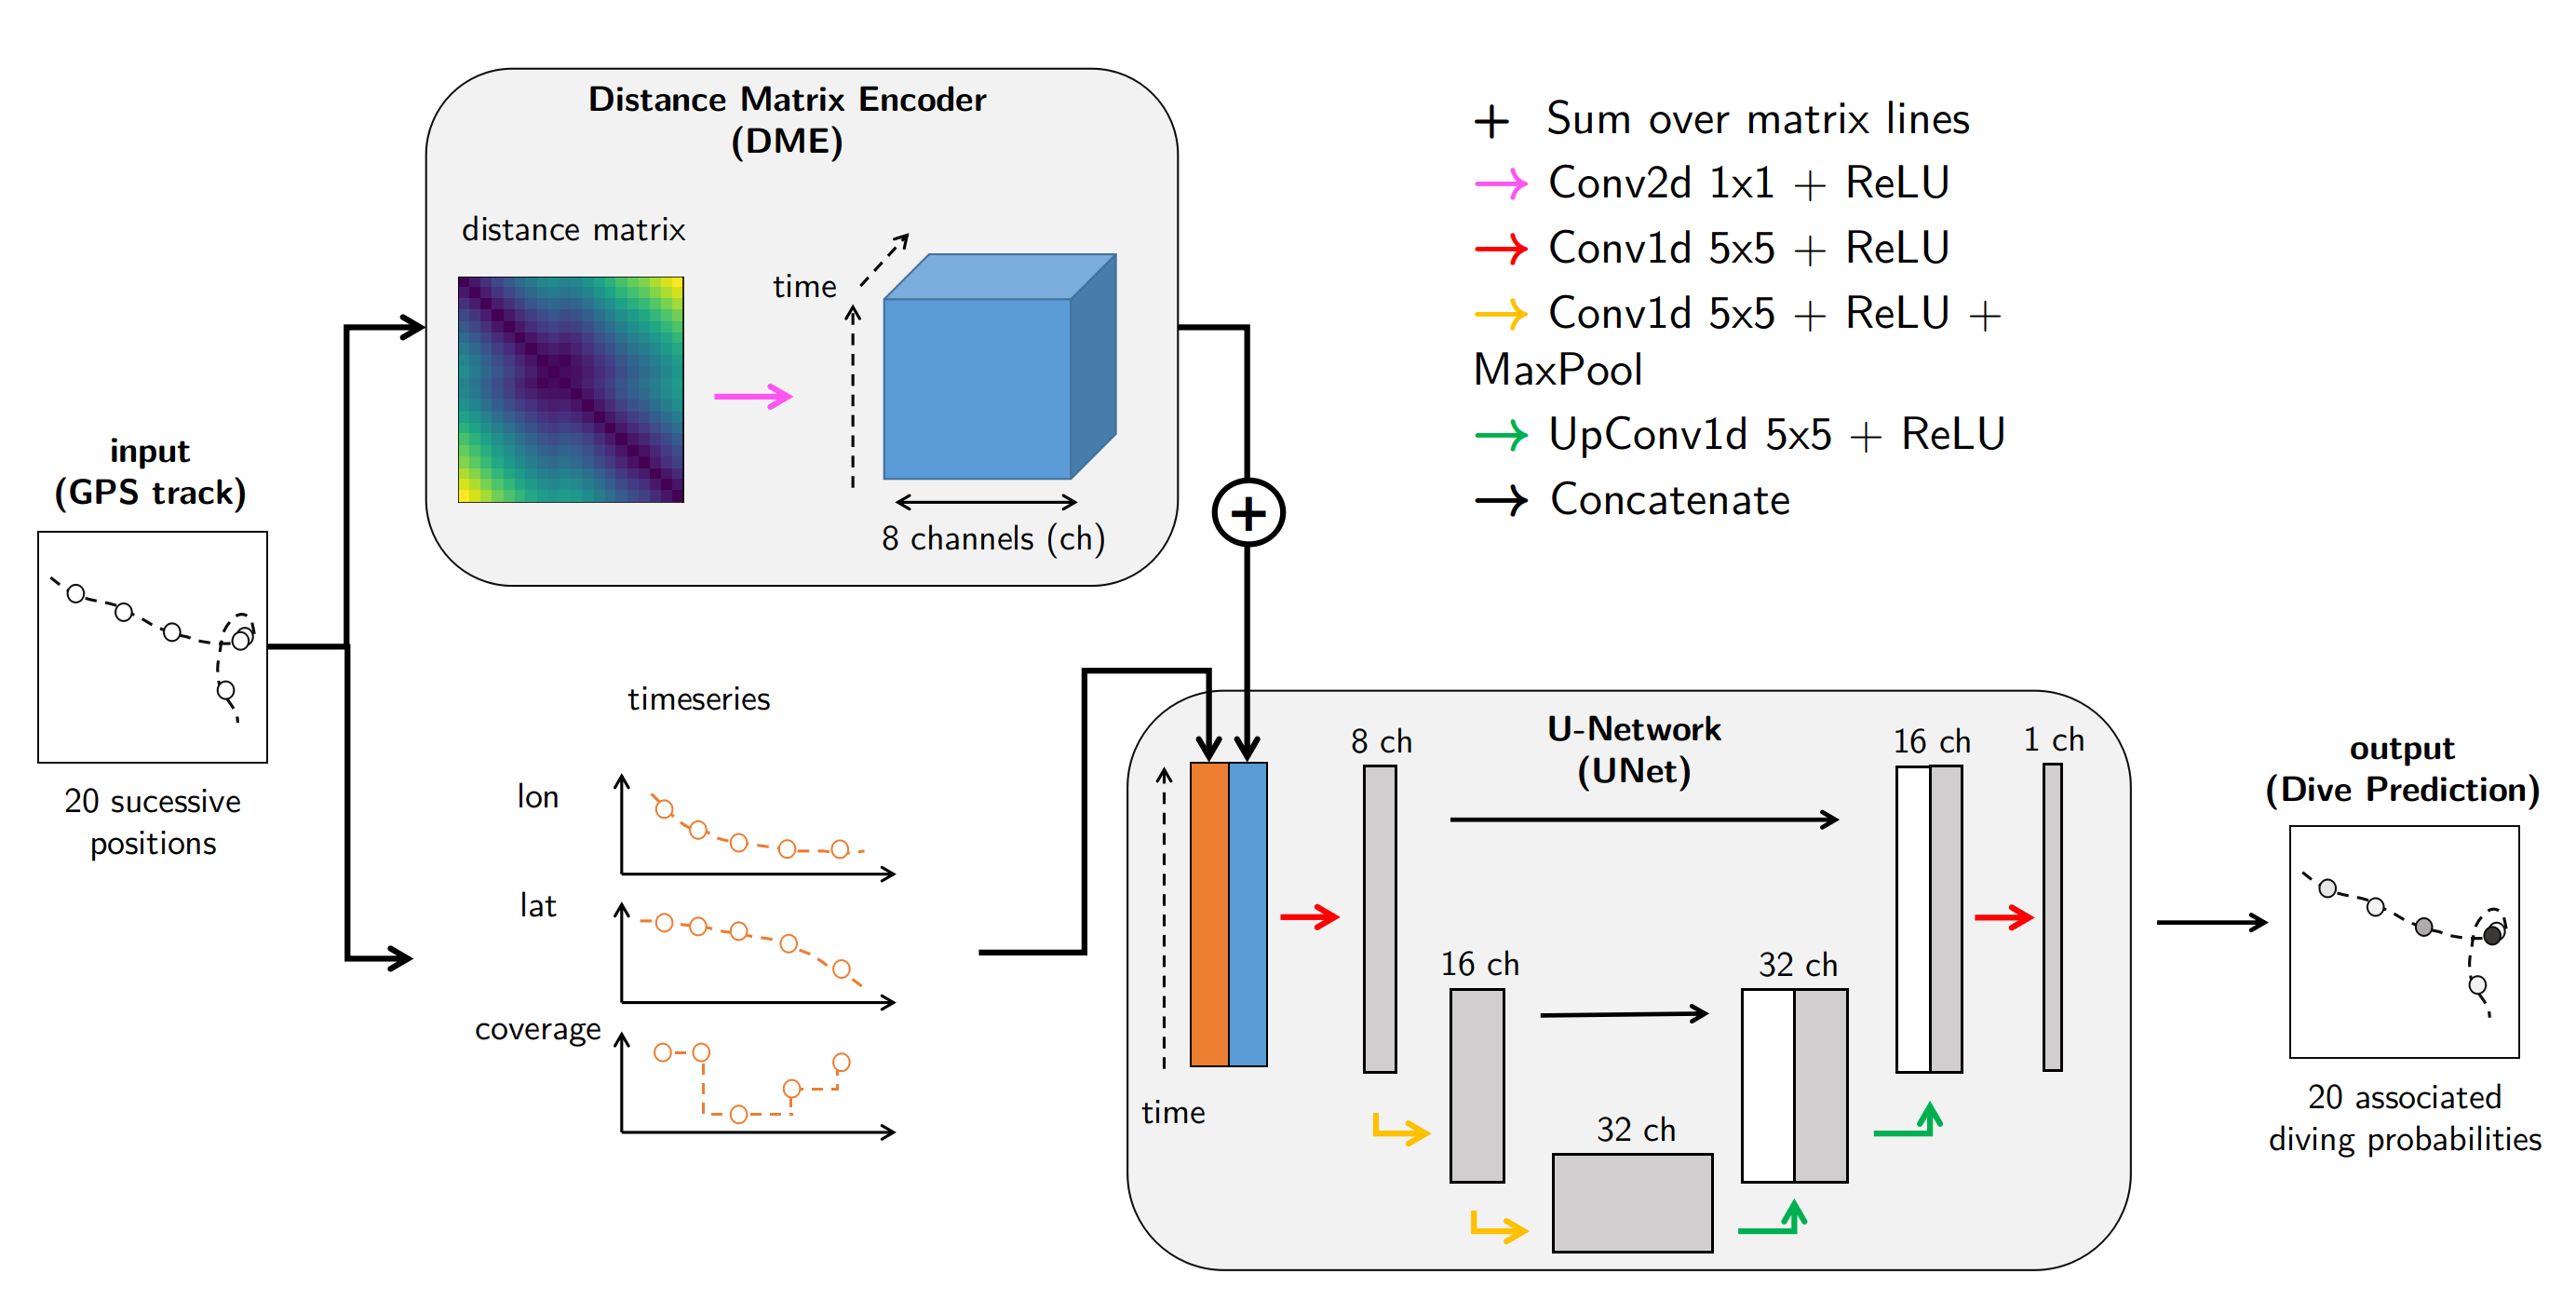
\includegraphics[scale=0.45]{figure3.png}
  \caption{\textbf{DME-UNet Architecture} - This network is composed of two blocks entitled Distance Matrix Encoder (DME) and U-Network (UNet). It takes as input a GPS of 20 successive positions and outputs a diving probability to each of these positions. A channel refer to deep learning terminology and describes a representation of the input data as output of some computation layer. Conv1d, Conv2dn MaxPool, and UpConv1d are abbreviations for usual deep learning operations in convolutional networks. Details can be found on pytorch's documentation \cite{paskze_pytorch_2019} }
  \label{figure3}
\end{figure}


The DME takes as input a distance matrix.
This distance matrix is simply obtained by computing the orthodromic distance between each pair of positions in the input track. Its lines and rows are ordered in increasing time.
The idea behind this representation of trajectory data is that longitude and latitude time-series may not be the best representations for neural-network-based methods since movement trajectories inherently contain 2D spatial information which might not be easily perceivable in simple time-series.
The performance of machine learning methods is heavily dependent on the choice of data representation (or features) on which they are applied \cite{bengio_representation_2014}. We expect the distance matrix representation to better encode 2D spatial patterns along a trajectory.
Given a matrix distance, the DME applies a 2-dimensional convolutionnal layer with 8 channels (i.e. 8 output features) combined with rectifier linear unit activations.
As a feature extraction step, we then sum the resulting output over the horizontal direction to extract a 8-dimensional feature vector at each position of the considered trajectory segment.
In short, this network can be regarded as a trainable function that would compute residence time defined as in \cite{barraquand_animal_2008}, but with circle of different radius which values will be adjusted automatically by the network.

We adapt a U-Net architecture, which is the state-of-the-art neural architecture for segmentation tasks \cite{ronneberger_u-net_2015}, to a multivariate 1-dimensional setting.
As inputs, we provide the U-Net with a 11-dimensional time series which concatenate the raw longitude, latitude and coverage ratio time series and the output of the DME. The key feature of the U-Net architecture is to combine the information extracted by convolutional blocks applied at temporal scales. To achieve this multi-scale analysis, the U-Net applies pooling layer to coarsen the time resolution and interpolation layers (UpConv1d layers) to increase the time resolution as sketched in Fig.\ref{figure3}. At each scale, we apply a specific convolution block. We concatenate its output with the interpolated output of the coarser scale to a convolutional block, whose output is interpolated to the finer resolution. Overall, we may notice that the output of the U-Net architecture is a time series with the same time resolution as the input time series. Similarly to the fully-connected architecture, the last layer applies a sigmoïd activation to transform the output into a time series of diving probabilities. Overall, this architecture (DME + U-Net) involves $2.10^{4}$ parameters which is approximately 30 times less than for the FCNet.

\subsubsection{Network Training and Validation}
Given a selected neural network architecture, the training procedure relies on a supervised learning scheme using a weighted binary cross entropy as loss function.
This function evaluates the performance of a prediction by comparing the dive prediction (output of the model) with the true dives defined by TDR data. We consider a weighted version of the binary cross entropy because of the unbalanced presence of dive and no-dive behaviour in the studied trajectories (see Table \ref{table1}). The objective is to penalize more  for mistakes on the smaller class (diving behaviour) than for false positive, thus ensuring for convergence. In the reported experiments, the weight was empirically set to 5 for cormorants datasets and 30 for boobies dataset.

The minimisation of the training loss exploits the  Adam stochastic optimizer \cite{kingma_adam_2014}.
Networks were evaluated on training and validation datasets every epoch (defined as one pass through the entire train dataset). We consider an early-stopping criterion such that the training procedure was stopped as soon as the validation loss started increasing.
Overall, given a trajectory the diving probability at a given location was assessed by computing the mean probability of all predictions derived from all 20 positions windows.
These models were implemented, trained and tested with python using pytorch library \cite{paskze_pytorch_2019}. Our pytorch Code is available on our github repository: https://github.com/AmedeeRoy/BirdDL.

\subsection{Benchmarked methods}
Two classical methods for dive prediction First-Passage Time (FPT), and Hidden Markov Models (HMM) were evaluated for intercomparison purposes.
FPT was computed following \cite{fauchald_using_2003}, by selecting the radius that maximizes the variance of passage times. Time passage values were converted into a probability of dives with min-max normalization.
Regarding HMMs, we applied the momentuHMM R package \cite{mcclintock_momentuhmm_2018}. We implemented HMMs with 3 behavioural modes associated to traveling, searching and diving behaviours. This approach represents trajectories as a sequence of steps and angles. It models steps as random variables following a gamma marginal distribution and angle following a von mises marginal distribution.
In this HMM setting, the coverage data was used as covariate in the transition probability matrix, assuming that low coverage ratio might provide a proxy of the likelihood of the diving behaviour and vice-versa. We may point out that the HMMs direclty provide as outputs a likelihood value of the diving behaviour.

\subsection{Evaluation scheme}
We describe below the evaluation scheme we implemented to assess the performance of the proposed neural network approaches. We first focuses on the benchmarking of the performance of the considered approaches in terms of dive prediction accuracy. For the proposed neural network architectures, we further analyze the impact on the dive prediction performance of different data types used as inputs as well as their generalization performance.

\paragraph{Dive prediction performance}
As evaluation metrics for dive prediction, we evaluated the receiver operating characteristics curve (ROC), the area under the curve (AUC) as well as the binary cross entropy (BCE) for the test datasets.
For binary classification, the ROC curve plots the true positive rate (i.e. true predicted dives) against the false positive rate (i.e. false predicted dives). We obtain this curve by varying the probability threshold defining dive/no dive behaviours. Regarding the AUC, it was estimated by integrating the ROC curve along the x axis using the composite trapezoidal rule. For neural network approaches, we also analyzed the value of training loss for the training and test datasets.

\paragraph{Data inputs}
Both studied species breed in the most productive upwelling system, the Humboldt Current System (HCS) and feed on the same preys, i.e. Peruvian anchovies \cite{jahncke_diets_1998}. However, they are known to have distinct foraging strategies: boobies are plunge divers reaching in average about 2 m depth and spending most of the time in fly, while cormorants dive deeper and longer in average, reach up to 30 m depth, and spend up to 40\% of the time in water \cite{weimerskirch_foraging_2012}.
We assessed the dive prediction performance of the benchmarked methods when considering trajectory data derived from these two distinct seabird and associated with different time resolutions, more precisely trajectory data sampled at 5, 15 and 30s.
We specifically evaluated the relative importance of coverage data and of the Distance Matrix Encoder by training neural network approaches with and without this information. As mentioned above, we also applied the HMM with and without coverage data used as covariate in the transition probability matrix.
Overall, this led to the quantitative comparison of the performance of 17 models and 6 datasets all listed in Table \ref{table2}.

\begin{table}[h]
 \caption{\textbf{Overview of all Trained Deep Networks} - All trained deep networks on the trajectories of Pescadores are given in this table, plus other methods used for comparison. AUC means the Area Under the ROC curve, BCE is for binary cross entropy computed on the testing trajectories. Train and Validation Loss correspond to the loss estimation after model training on respectively training and validation trajectories. SV is for Peruvian boobies (\textit{Sula variegata)}, LB is for Guany cormorants (\textit{Leucocarbo bougainvilli})}
  \centering
  \begin{tabular}{llllllll}
    \toprule
    Dataset  &  Resolution &  Model & Variables & AUC & BCE & Train Loss & Validation Loss \\
    \midrule
    SV       & 5s  & FPT    & lon, lat               & 0.76 & 1.09 & - & -     \\
(Pescadores) &     & HMM    & step length, direction & 0.87 & 2.98 & - & -     \\
            &     & HMM    & step length, direction, cov & 0.88 & 2.83 & - & - \\
             &     & FCNet  & lon, lat               & 0.71 & 0.52 & 1.05 & 1.12 \\
             &     & FCNet  & lon, lat, cov          & 0.94 & 0.22 & 0.42 & 0.74  \\
             &     & UNet   & lon, lat               & 0.72 & 0.48 & 0.97 & 1.12  \\
             &     & UNet   & lon, lat, cov          & 0.96 & 0.21 & 0.47 & 0.61  \\
             &     & DME-UNet   & lon, lat   & 0.92 & 0.27 & 0.57 & 0.66  \\
             &     & \textbf{DME-UNet}   & \textbf{lon, lat, cov}  & \textbf{0.97} & \textbf{0.16} & \textbf{0.36} & \textbf{0.56}  \\
             & 15s & FPT    & lon, lat               & 0.76 & 1.49 & - & -      \\
             &     & HMM    & step length, direction, cov & 0.89 & 3.36 & - & -       \\
             &     & FCNet  & lon, lat, cov          & 0.76 & 0.94 & 1.65 & 1.80 \\
             &     & \textbf{DME-UNet}   & \textbf{lon, lat, cov}  & \textbf{0.92} & \textbf{0.45} & \textbf{0.86} & \textbf{1.07}  \\
             & 30s & FPT    & lon, lat               & 0.78 & 1.93 & - & -      \\
             &     & \textbf{HMM}    & \textbf{step length, direction, cov} & \textbf{0.88} & \textbf{1.91} & \textbf{-} & \textbf{-}       \\
             &     & FCNet  & lon, lat, cov          & 0.76 & 1.30 & 2.13 & 2.40 \\
             &     & DME-UNet   & lon, lat, cov  & 0.87 & 0.82 & 1.32 & 1.52 \\
    \midrule
    LB       & 5s  & FPT    & lon, lat               & 0.73 & 5.2 & - & -        \\
(Pescadores) &     & HMM    & step length, direction, cov & 0.78 & 7.10 & - & -      \\
             &     & FCNet  & lon, lat, cov          & 0.92 & 0.44 & 0.44 & 0.47  \\
             &     & \textbf{DME-UNet}   & \textbf{lon, lat, cov}  & \textbf{0.95} & \textbf{0.36} & \textbf{0.38} & \textbf{0.39}  \\
             & 15s & FPT    & lon, lat               & 0.77 & 5.7 & - & -      \\
             &     & HMM    & step length, direction, cov & 0.81 & 4.76 & - & -  \\
             &     & FCNet  & lon, lat, cov          & 0.94 & 0.41 & 0.53 & 0.51  \\
             &     & \textbf{DME-UNet}   & \textbf{lon, lat, cov}  & \textbf{0.95} & \textbf{0.35} & \textbf{0.40} & \textbf{0.43}  \\
             & 30s & FPT    & lon, lat               & 0.79 & 6.0 & - & -      \\
             &     & HMM    & step length, direction, cov & 0.86 & 4.26 & - & - \\
             &     & FCNet  & lon, lat, cov          & 0.91 & 0.65 & 0.84 & 0.79  \\
             &     & \textbf{DME-UNet}   & \textbf{lon, lat, cov}  & \textbf{0.96} & \textbf{0.57} & \textbf{0.63} & \textbf{0.62}  \\
    \bottomrule
  \end{tabular}
  \label{table2}
\end{table}

\paragraph{Generalization properties}
When considering neural network approaches, training models which may apply beyond the considered training framework is a key feature, generally referred to as the generalization performance of the trained neural networks. Here, we evaluated this generalization performance through the application of models trained on Pescadores dataset to the Gua\~nape dataset.
This dataset is composed of Peruvian boobies trajectories but from a different breeding colony. Beyond the different in the case-study region, we expect peruvian boobies behaviour to share common features across colonies, so that models fitted to the trajetory data of a given colony might still be meaningful when applied to another colony.
In this experiment, we compared the dive prediction performance of FPT and HMM methods to the best FCNet and DME-UNet models. Beyond AUC and BCE performance metrics, we also evaluated the relevance of the estimated map of dive distributions. The later were computed using a weighted Kernel Density Estimator (KDE) using dive probabilities as weighing factor. As groundtruth, we considered the map of dive distributions estimated from true dive locations defined by TDR data. From these maps, we evaluated an Hellinger distance as an integrated performance metrics for the different approaches \cite{wilson_distancebased_2011}.

\section{Results}

We detailed below the numerical experiments performed in this study to assess the relevance of the proposed neural network approaches to predict dive behaviour of Peruvian boobies and cormorants from trajectory data.

\paragraph{Overall performance}
For all datasets, the different methods obtained contrasted performance results, with AUC going from 0.71 to 0.97 (see Table \ref{table2}), which corresponds in the best cases to correct prediction rates of diving and non-diving behaviour of approximately 90\% and of 70\% in the worst cases (see Figure \ref{figure1}). Overall, neural networks-based approaches obtained better performance than the state-of-the art methods, with highest AUC (around 0.9) and lowest binary cross entropy (around 0.5). First-Passage Time obtained quasi systematically the lowest AUC, and the Hidden Markov Models had most of the time AUC around 0.85 but the highest BCE. State-of-the-art methods were outperformed by neural networks specifically for the 5s resolution datasets, with AUC improvements up to 15\% with neural networks over HMM. In particular, the DME-UNet was the most consistent method, being able to get better performance on most datasets, and to improve substantially the performance of the FCNet proposed by \cite{browning_predicting_2018}. As illustration, on the boobies dataset, BCE was approximately two times lower with the DME-UNet than with the FCNet, and the DME-UNet obtained systematically higher AUC.

\begin{figure}[!h]
  \centering
  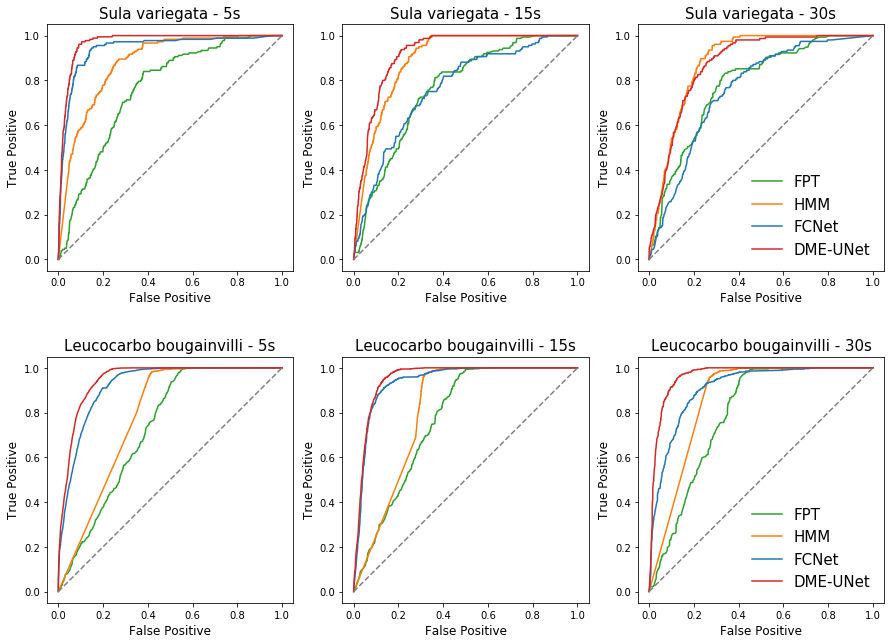
\includegraphics[scale=0.5]{figure1.png}
  \caption{\textbf{Comparison of algorithms} - ROC curves obtained from the prediction of 4 algorithms, First-Time Passage (FPT), 3-states Hidden Markov Models (HMM), Fully-Connected Network (FCN) and U-Network with a Distance Matrix Encoder (DME-UNet) on 4 distinct test datasets derived from two seabirds species breeding in Pescadores Island from 2008 to 2013}
  \label{figure1}
\end{figure}

\paragraph{Impact of the temporal resolution}
Interestingly, on the cormorant dataset the sampling resolution did not affect much the performance of the neural network approaches (DME-UNet with AUC of 0.95) whereas state-of-the-art methods FPT/HMM had increasing AUC with larger resolution going from respectively 0.73/0.78 to 0.79/0.86 (see Table \ref{table2}).
At the opposite, on the peruvian datasets the FPT/HMM methods had constant performance disregarding the sampling resolution (AUC around 0.76/0.88), while deep learning tools had decreasing AUC with larger resolution. In particular, the dataset of Peruvian boobies with the larger resolution (i.e. 30s) is the only one where neural networks did not do any better than state-of-the-art. Yet, if DME-UNet's performance are pretty much equivalent to the highest AUC obtained by HMM (AUC of 0.87), on this dataset the FCNet had lowest prediction performance (AUC of 0.76) (see Figure \ref{figure1}).

\paragraph{Impact of data inputs}
Deep networks had substantial increase of accuracy through the coverage ratio data, all three networks FCNet, UNet and DME-UNet having very high prediction accuracy with AUC around 0.95 (see Table \ref{table2}) .
Yet, without coverage information, accuracy was way poorer with AUC around 0.7, except for the network using a Distance Matrix Encoder (DME-UNet) that maintains an AUC at 0.92.
At the opposite, the removal of coverage data did not change significantly the performance indexes of the HMM with a relatively constant AUC of 0.87 (see Figure \ref{figure2}).

\begin{figure}[!h]
  \centering
  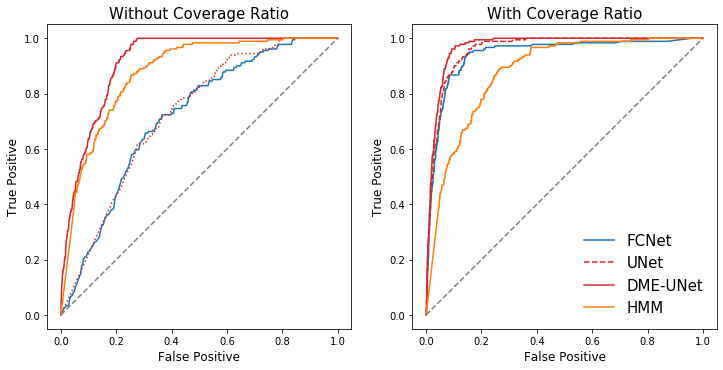
\includegraphics[scale=0.5]{figure2.png}
  \caption{\textbf{Comparison of data inputs} - ROC curves obtained from the prediction of 3 deep networks, Fully-Connected Network (FCN) and U-Network with/without a Distance Matrix Encoder (resp. UNet / DME-UNet) on the test dataset derived from Peruvian boobies sampled at 5s breeding in Pescadores Island from 2008 to 2013}
  \label{figure2}
\end{figure}


\paragraph{Maps of diving probabilities}
We further analysed the relevance of the dive predictions through the estimated dive distributions maps reported in Figure \ref{figure4a} and \ref{figure4b}. For both species, we can observe neural networks and HMM approaches have contrasted outputs (either very high or low diving probabilities), while the FPT approach is the one that discriminate the least dive from non-diving behaviours. Moreover, these maps also point out that from all methods false positive are predicted with high probabilities in areas where no true dives occurred (i.e. isolated blue circle with high radius). Yet, it is particularly visible from FCNet and HMM output and specifically in the vicinity of the colony.

\newpage

\begin{figure}[!h]
  \centering
  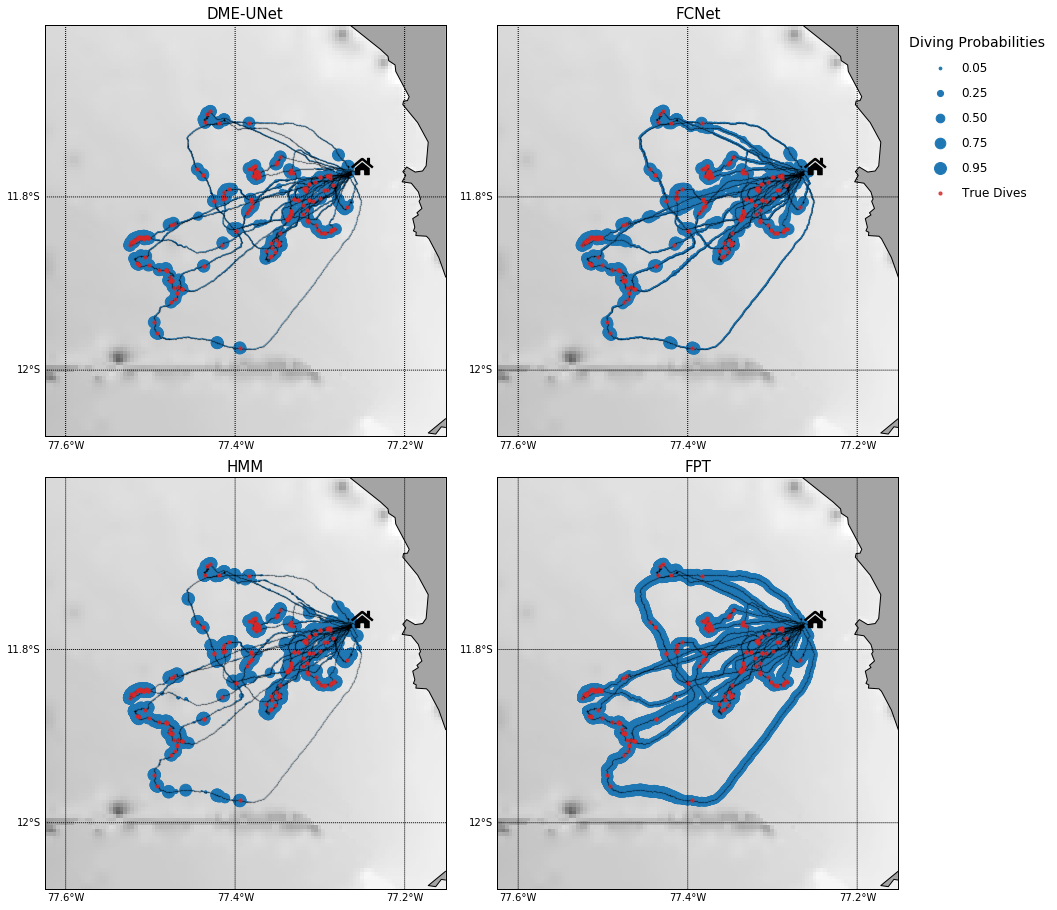
\includegraphics[scale=0.5]{figure4a.png}
  \caption{\textbf{Maps of Peruvian boobies predicted dives} - Maps of the trajectories. Red points represent true dive derived from TDR data. Blue points represents diving probabilities of each location with radius increasing for higher probabilities. These probabilities are the results of four methods on the same Dataset (SV 5s), with our proposed network DME-UNet (top left), the fully connected network used by \cite{browning_predicting_2018}  FCNet (top right), the 3 states Hidden Markov Models HMM (bottom left), and the First Time Passage apporach FPT (bottom right)}
  \label{figure4a}
\end{figure}

\begin{figure}[!h]
  \centering
  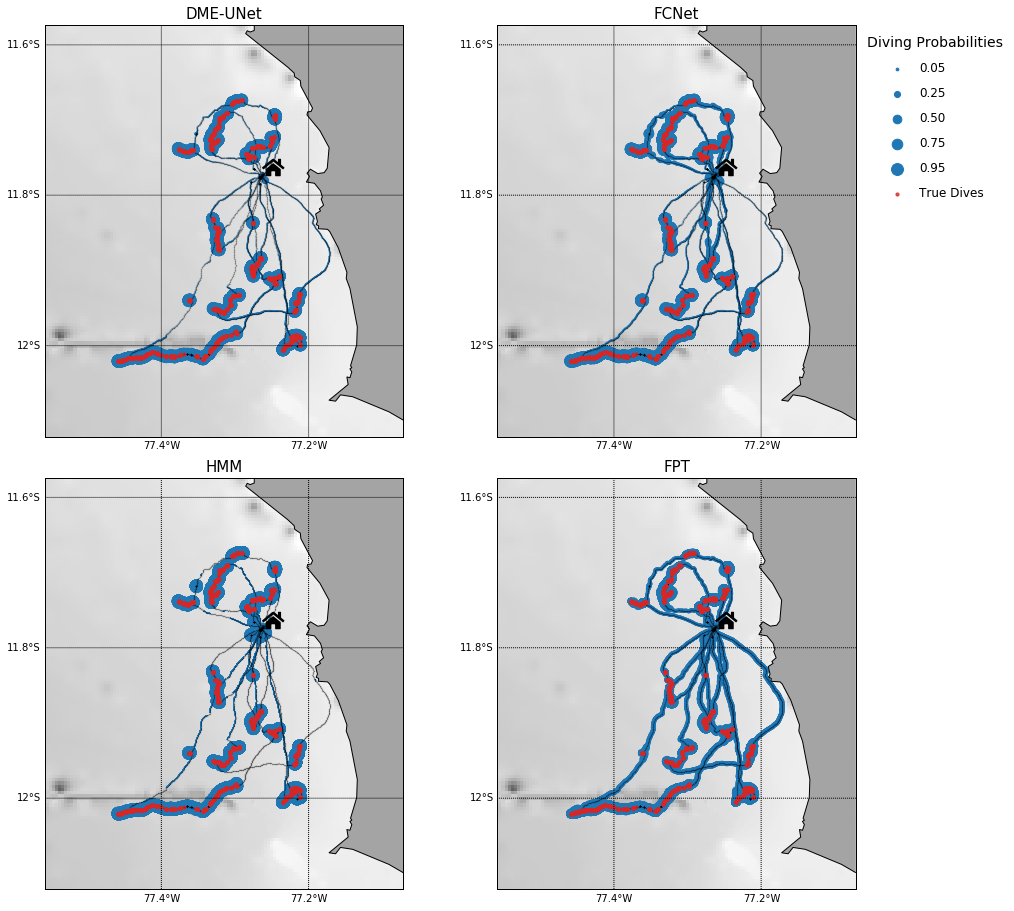
\includegraphics[scale=0.5]{figure4b.png}
  \caption{\textbf{Maps of Guanay cormorants predicted dives} - Maps of the testing trajectories. Red points represent true dive derived from TDR data. Blue points represents diving probabilities of each location with radius increasing for higher probabilities. These probabilities are the results of four methods on the same Dataset (LB 5s), with our proposed network DME-UNet (top left), the fully connected network used by \cite{browning_predicting_2018}  FCNet (top right), the 3 states Hidden Markov Models HMM (bottom left), and the First Time Passage apporach FPT (bottom right)}
  \label{figure4b}
\end{figure}

\newpage

\paragraph{Application to Gua\~nape dataset}
The use of deep networks trained on the dataset of Peruvian boobies from Pescadores Island on trajectories from birds from another colony (i.e. Gua\~nape) revealed once again the higher accuracy of deep learning based algorithms (see Figure 3). Both FCNet and DME-UNet outperformed HMM and FPT in terms of AUC (e.g., with AUC of around 0.97 for neural networks vs. 0.88 for HMM). The Hellinger distance of the estimated dive distribution maps stressed the greater relevance of DME-UNet predictions with a distance value 1.6 times smaller than the one derived from FCNet estimations and 2 times smaller than the one derived from HMM estimation.


\begin{table}[h]
 \caption{\textbf{Gua\~nape projection} - The deep network fitted on the 5s sampled SV dataset in Pescadores have been used for dive prediction in Gua\~nape. AUC is for area under the roc curve. BCE is the binary cross entropy. Hellinger Distance corresponds to the distance of the diving distribution maps estimated with kernel density estimations and plotted in Figure \ref{figure5} to the correct diving distribution. SV is for Peruvian boobies (\textit{Sula variegata)}}
  \centering
  \begin{tabular}{llllllll}
    \toprule
    Dataset  &  Resolution &  Model & Variables & AUC & BCE & Hellinger Distance \\
    \midrule
    SV      & 5s  & FPT    & lon, lat               & 0.78 & 0.93 & 31.7          \\
  (Gua\~nape) &     & HMM    & step length, direction, cov & 0.88 & 3.70 & 29.6     \\
            &     & FCNet  & lon, lat, cov  & 0.97 & 0.10 & 25.0                  \\
            &     & DME-UNet   & lon, lat, cov  & 0.96 & 0.07 & 15.1              \\
    \bottomrule
  \end{tabular}
  \label{table3}
\end{table}


\begin{figure}[!h]
  \centering
  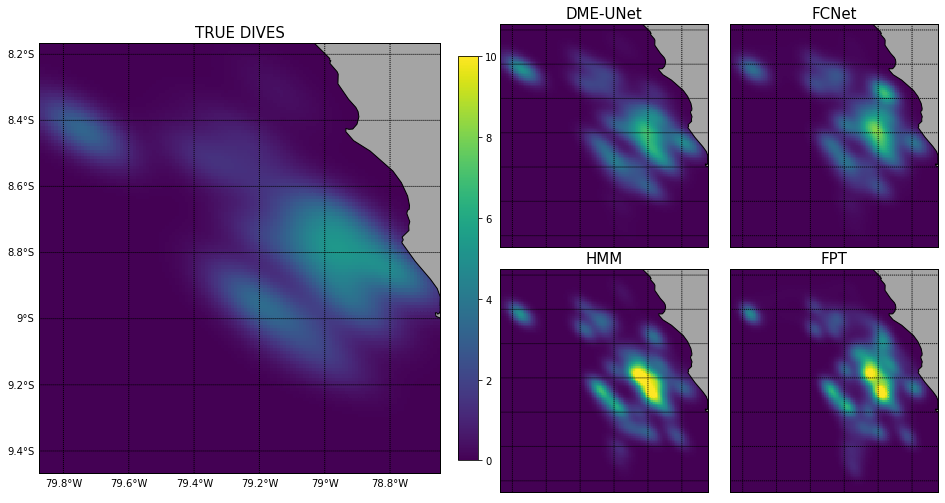
\includegraphics[scale=0.5]{figure5.png}
  \caption{\textbf{Maps of dive distributions of Peruvian Boobies from Gua\~nape Island} - These density maps were obtained through Kernel Density Estimation. The left map has been computed from true dives derived from TDR data. The four other maps are estimations of this map, using  all points of the trajectories with weights associated to diving probabilities estimated by the four studied approaches,  with our proposed network DME-UNet (top left), the fully connected network used by \cite{browning_predicting_2018}  FCNet (top right), the 3 states Hidden Markov Models HMM (bottom left), and the First Time Passage apporach FPT (bottom right). Hellinger distance of the 4 estimations to the ground truth defined as the TRUE DIVES map are in Table \ref{table3}}
  \label{figure5}
\end{figure}

\section{Discussion}
This study aimed at predicting seabirds dives from GPS data only by training a deep network in a supersized manner based on TDR data to define the true dives.
In line with \cite{browning_predicting_2018}, this study further  supports the relevance of deep learning approach over classical methods for dive predictions.
Moreover, we introduce a new deep network, the so-called DME-UNet, which combines a state-of-the-art deep network architecture with a meaningful geometrical representation of trajectory data. We reported even better results with higher stability to the different data inputs.

The proposed network allows not only to better predict dive behaviour but also results in better seabird dive distribution maps. Recently numerous studies used seabirds dive as a proxy for prey distribution, and such distribution are usually computed by applying KDE on dive predictions derived from HMMs \cite{delord_movements_2020,weimerskirch_at-sea_2020,zhang_gps_2019}.
Here, we show that the error in the estimation of dive distributions maps can be divised by two by using deep learning tools rather than HMM tools.
In our specific study, HMMs have over-estimated the frequency of dives at proximity of breeding locations. Sulids and cormorants  spend  time  bathing  near their breeding territories involving vigorous splashing and beating the water with the wings, \cite{nelson_pelicans_2005}. Such behaviours associated to low speed might be erroneously classified as diving behaviour by HMMs which could explain the observed bias. For the same reason, we might explain that HMM are better on the boobies dataset than with cormorants because these birds spend more time resting at the surface, which corresponds to low speeds without being dives (see Table \ref{table1}). The high BCE obtained by HMM also suggests that in these situations HMM predicts erroneously dive with high confidence.
In opposition, deep learning seem better for discriminating such resting/bathing behaviours from dives. It would be nice to see further why and how deep networks succeed in outperforming HMMs, but the interpretation is one of the inherent difficulty  of deep learning. Not that it is not possible, but that it would require further analysis. Yet, having such results on deep networks performance over HMM is a first step in the demonstration that there is some information that the HMMs misses and that it can be captured by deep networks.

As shown in Figure \ref{figure1}, the better performance reported with DME-UNet closely related to the temporal resolution of the sampled dataset.
In particular, from Peruvian boobies' trajectories resampled at 15s and 30s, similar results were obtained through DME-UNet and HMM. However, we observed that with the 5s resolution dataset, deep networks had outperformed HMM. This suggests that HMMs are great approaches to trajectory segmentation with relatively large temporal resolution, and that they are unable to interpret movement process at very fine spatio-temporal scales as well as deep networks do. Knowing that Peruvian boobies dive during very short periods, approximately 2 seconds (see Table \ref{table1}), this suggests that the deep networks would be able to capture diving behavioural movements from a GPS track sampled with a resolution in the same order of magnitude than dive durations.
For the Guanay cormorants dataset, DME-UNet had better results than HMM for all tested sampling resolution. However, cormorants dives last about 20s, which could explain why even with the 30s sampled dataset deep networks had better results than HMMs. We might infer that a decrease of the performance of deep networks would occur for sampling resolution of 1 minute or more.
With technological advances in sensor technology, ecologists are able to collect larger amount of data than ever before. We might expect GPS with lower consumption, higher resolution in the future. Such an expected trend would make more critical the exploitation of development of the proposed deep learning approaches to make the most of the collected high-resolution  animal trajectories   \cite{beyan_setting_2020,malde_machine_2020, yoda_advances_2019}

The GPS tracks were characterized by short gaps in the regularly sampled sequence of locations, since these devices do not receive a satellite signal while submerged \cite{boyd_movement_2014,wilson_technological_2012}.
These gaps are therefore sometimes directly considered indicative of diving behaviour \cite{weimerskirch_foraging_2012}.
Surprisingly, HMM did not take benefits from such variable for inferring dives.
Nevertheless, the use of this coverage information as input helped substantially deep networks to predict dives.
Indeed, without coverage data, the FCNet proposed by \cite{browning_predicting_2018} predicted dives with relatively low accuracy, with in particular AUC of 0.71 which is low  compared to HMMs' performance (AUC of 0.87), while it obtained AUC of 0.94 using this external information (see Figure \ref{figure2}). In their study, Browning et al. also used in some cases altitude data to get better performance than HMM. One could therefore argue that deep networks are not relevant with longitude and latitude data only.
However, the DME-UNet proposed in this study demonstrated the ability of deep networks to classify animal behaviours in such situation. Indeed, without the coverage ratio variable it obtained still an AUC of 0.92 which was about 5 \% more than HMM. This demonstrates that this approach is not only relevant for seabirds where coverage ratio is an important external variable, but also for any trajectory dataset.

A key breakthrough of our approach was thus to use what we called a Distance Matrix Encoder (DME), which is a simple neural network block which aims to extract features for a better geometrical description of a trajectory.
The performance of machine learning methods is heavily dependent on the choice of data representation (or features) on which they are applied \cite{bengio_representation_2014}.
Most studies dealing with trajectory data represented movement with longitude and latitude time-series. Yet, some studies argued that such representation might not be relevant for neural-network based methods since movement trajectories inherently contain 2D spatial information which might not be easily perceivable in simple time-series. For instance, previous works  investigated one-hot representations initially introduced for text data  \cite{nguyen_geotracknet-maritime_2021} as well as trajectory image \cite{endo_classifying_2016}. Here, we explored distance matrix representations as the distance matrix of positions has been shown to capture relevant spatial information for protein structure prediction \cite{senior_improved_2020, xu_analysis_2019}. Our study  demonstrates its relevance when considered as input to a neural network architecture to complement longitude and latitude time series. Future work may further investigate how distance matrix representation could be of interest for other deep learning approaches to trajectory data, including among others Recurrent Neural Network (RNN), and Generative Adversarial Networks (GAN) for trajectory prediction and simulation \cite{ardakani_encoding_2017,goodfellow_generative_2014,isola_image--image_2018,rew_animal_2019}.


When considering learning-based schemes, the assessment of the generalization performance is of key importance. Beyond the evaluation of dive prediction performance on a trajectory dataset, which is independent from the training dataset, the question whether a model trained on a given dataset, e.g. for a given species, colony and time period, may apply to other species, colonies and/or time periods, naturally arises as a key question. Numerous studies in the deep learning literature \cite{kawaguchi_generalization_2020,zhang_understanding_2017} have highlighted that some neural architectures show relevant generalization properties whereas others may not.
Here, we evaluated the generalization performance of the benchmarked methods for two colonies of Peruvian boobies.
Peruvian boobies from  Gua\~nape Island did have different foraging strategies from their counterparts from Pescadores island, with trips two times longer and dives slightly longer (see Table \ref{table1}). It turned out that the two deep networks were very stable on this testing dataset predicting dives with high accuracy (AUC of 0.97). The improvement of neural networks over the HMM fitted to the dataset was about 10\%.
These results support the relevance of deep learning schemes as
'ready-to-use' tools which could be used by ecologists to predict
seabirds dives on new datasets. To make easier such applications, we share online the different models we pre-trained on the considered dataset (https://github.com/AmedeeRoy/BirdDL/results).
Beyond such a direct application, trained models may also be of key interest to explore transfer learning strategies, which refer to the ability of exploiting some previously trained models to address a new task or dataset rather than training a new model from scratch. Fine tuning is a typical example of transfer learning procedure. It uses a previously trained model as the initialization of the training scheme. Such a strategy may be particularly relevant when the training dataset may not be sufficiently large to train a model from scratch. We then expect the models trained in this work to be potentially of interest for the fine-tuning of these models on datasets referring to other colonies and species of same genus.

\subsection*{Acknowledgements}
We thank all people involved in fieldworks: H. Weimerskirch, K. Delord, C. Barbraud, Y. Tremblay, J. Silva, G. Passuni, C. Boyd and C. Saraux. We thank Proabonos for permission to work on Isla Gua\~nape  and Isla Pescadores.

\subsection*{Funding statement}
This work is a contribution to the TRIATLAS project (European Union's Horizon 2020 research and innovation program – grant agreement No. 817578), and to the Young Team IRD Programm (JEAI) for TABASCO project. RF was supported by LEFE program (LEFE MANU project IA-OAC), CNES (grant SWOT-DIEGO) and ANR Projects Melody and OceaniX. Fieldworks have been conducted thanks to the cooperative agreement between IRD, the Agence Nationale de la Recherche (ANR) project TOPINEME, and of the International Joint Laboratory DISCOH.

\subsection*{Ethics statement}
Foraging trip routes and dive depth data were obtained from electronic devices attached to Peruvian Boobies and Guanay Cormorants tagged at the Pescadores  Gua\~nape Islands, Peru, from 2007 to 2013. Capture, restraint, holding and release of birds for attachment and subsequent removal of electronic devices were performed under the auspices of institutional animal use and care a Peruvian federal agency, Programa de Desarrollo Productivo Agrario Rural, commonly known as “Agrorural”. Headquarters of Agrorural are located at Av. Salaverry 1388, Lima, Peru. Protocols for care and use of subject birds were reviewed and approved by Agrorural officials prior to every fieldwork sessions.


\printbibliography

\newpage

\end{document}
